\themaD
\graphicspath{{../../S22_Le_ratio/Images/}}

\chapter{Le ratio}
\label{S22}


%%%%%%%%%%%%%%%%%%%%%%%%%%%%%%
%%%%%%%%%%%%%%%%%%%%%%%%%%%%%%
\begin{autoeval}
   \small
   \begin{enumerate}
      \item Il partage une quantité en deux ou trois parts selon un ratio donné.
   \end{enumerate}
\end{autoeval}

\begin{prerequis}
   \begin{itemize}
      \item Notion de ratio.
      \item[\com] Partager une quantité (par exemple une somme d’argent) en deux ou trois parts selon un ratio donné.
   \end{itemize}
\end{prerequis}

\vfill

\begin{debat}[Débat : d'où vient le ratio ?] 
   {\bf Ratio} vient de l’anglais {\bf ratio} que l’on traduit par proportion qui lui-même vient du latin {\bf ratio} qui signifie calcul ou compte. Ce vocabulaire est plutôt utilisé dans le monde anglo-saxon. \\
   On le retrouve pour la première fois dans {\it Les éléments}, d'{\it Euclide}, soit il y a environ 2\,300 ans !
   \begin{center}
       \begin{pspicture}(0,0)(7.5,4.7)
         {\psset{unit=0.35}
         \psgrid[subgriddiv=0,gridcolor=lightgray,gridlabels=0pt](0,0)(21,13)
          \psframe(0,0)(21,13)
          \psline(8,0)(8,13)
          \psline(0,8)(8,8)
          \psline(5,8)(5,13)
          \psline(5,10)(8,10)
          \psline(6,8)(6,10)
          \psline(5,9)(6,9)
          \psset{linecolor=B1,linewidth=0.2}
          \psarc(8,13){13}{-90}{0}
          \psarc(8,8){8}{180}{-90}
          \psarc(5,8){5}{90}{180}
          \psarc(5,10){3}{0}{90}
          \psarc(6,10){2}{-90}{0}
          \psarc(6,9){1}{90}{-90}}
      \end{pspicture}
   \end{center}
   \bigskip
   \begin{cadre}[B2][J4]
      \begin{center}
         Vidéo : \href{https://www.yout-ube.com/watch?v=vDZje8o_eD4}{\bf Quel est le point commun entre un ananas, des lapins et la tour de Pise ?}, chaîne {\it Unisciel}.
      \end{center}
   \end{cadre}  
\end{debat}


%%%%%%%%%%%%%%%%%%%%%%%%%%%%%%%%%%%
%%%%%%%%%%%%%%%%%%%%%%%%%%%%%%%%%%%
\activites

\begin{activite}[Représenter des ratios]
   {\bf Objectifs} :  calculer un ratio ; partager une quantité en deux ou trois parts selon un ratio donné.
   \begin{QCM}
      \begin{minipage}{7cm}
         {\psset{unit=0.8}
         \begin{pspicture}(-0.5,-0.5)(8,3.7)
            \psline(0,3)(0,0)(8,0)(8,3)
            \pscircle(1,0.5){0.5}
            \pscircle[fillstyle=solid,fillcolor=lightgray](2,0.5){0.5}
            \pscircle[fillstyle=solid,fillcolor=lightgray](3,0.5){0.5}
            \pscircle(4.5,0.5){0.5}
            \pscircle(5.5,0.5){0.5}
            \pscircle[fillstyle=solid,fillcolor=black](7,0.5){0.5}
            \pscircle(0.5,1.4){0.5}
            \pscircle[fillstyle=solid,fillcolor=lightgray](1.5,1.4){0.5}
            \pscircle(2.5,1.4){0.5}
            \pscircle(3.75,1.2){0.5}
            \pscircle[fillstyle=solid,fillcolor=black](5,1.4){0.5}
            \pscircle[fillstyle=solid,fillcolor=lightgray](6.25,1.2){0.5}
            \pscircle(7.5,1.4){0.5}
            \pscircle[fillstyle=solid,fillcolor=black](2,2.3){0.5}
            \pscircle(3.25,2.1){0.5}
            \pscircle[fillstyle=solid,fillcolor=lightgray](4.25,2.1){0.5}
            \pscircle(5.75,2.1){0.5}
            \pscircle(6.75,2.1){0.5}
            \pscircle[fillstyle=solid,fillcolor=black](5,2.8){0.5}
            \pscircle[fillstyle=solid,fillcolor=lightgray](3.75,3){0.5}
         \end{pspicture}}
      \end{minipage}
      \quad
      \begin{minipage}{9cm}
         Dans cette boite, il y a 4 balles noires pour 6 balles grises. \\
         On dit que la quantité de balles noires et grises est dans le ratio de 4 : 6 (on lit \og 4 pour 6 \fg{}) ou encore 2 : 3 (\og 2 pour 3 \fg{}). \\
   Inversement, le ratio des balles grises et noires est de 6 : 4.
      \end{minipage}
      \begin{enumerate}
         \item 
            \begin{enumerate}
               \item Quel est le ratio des balles noires et blanches ? Simplifier éventuellement ce ratio. \par \medskip
                  \pointilles \medskip
               \item Quel est le ratio des balles grises et blanches ? Simplifier éventuellement ce ratio. \par \medskip
                  \pointilles \medskip
               \item Comment pourrait-on écrire le ratio de balles noires, grises et blanches ? \par \medskip
                  \pointilles \medskip
               \item Quelle fraction du total des balles représente les balles noires ? Les balles grises ? Les balles blanches ? \par \medskip
                  \pointilles \medskip
            \end{enumerate}
         \item Dans cette question, on garde les mêmes ratios que dans les questions précédentes.
            \begin{enumerate}
               \item Si le bac contenait 40 balles, combien aurait-on de balles noires ? Grises ? Blanches ? \par \medskip
                  \pointilles \par \medskip
                  Quelle fraction du total des balles représente chaque sorte de balles ? \par \medskip
                  \pointilles \medskip
               \item Si le bac contenait 10 balles, combien aurait-on de balles noires ? Grises ? Blanches ? \par \medskip
                  \pointilles \par \medskip
                  Quelle fraction du total des balles représente chaque sorte de balles ? \par \medskip
                  \pointilles \medskip
               \item Si le bac contenait 130 balles, combien aurait-on de balles noires ? Grises ? Blanches ? \par \medskip
                  \pointilles \par \medskip
            Quelle fraction du total des balles représente chaque sorte de balles ? \par \medskip
                  \pointilles \medskip
            \end{enumerate}
         \item On souhaite partager 21 balles roses et violettes dans le ratio 3 : 4. Combien aura-t-on de balles roses et violettes ? \par \medskip
            \pointilles \medskip
        \item On partage 48 balles bleues, blanches et rouges dans le ratio 1 : 2 : 3. Combien a-t-on de balles de chaque couleur ? \par \medskip
         \pointilles \medskip
      \end{enumerate}
   \end{QCM}
\end{activite}


%%%%%%%%%%%%%%%%%%%%%%%%%%%%%%%%%%%
%%%%%%%%%%%%%%%%%%%%%%%%%%%%%%%%%%%
\cours 

%%%%%%%%%%%%%
\section{Définition du ratio}

\begin{definition}
   \begin{itemize}
      \item On dit que {\bf deux nombres} $a$ et $b$ sont, par exemple, dans le {\bf ratio} 3 : 4 si $\dfrac{a}{3} =\dfrac{b}{4}$. \\
         On parle de ratio \og trois pour quatre \fg. \\ [2mm]
         On peut le modéliser ainsi : \parbox{7cm}{\Ratio[FigureCours,Longueur=7cm,CouleurUn=DeepSkyBlue,CouleurDeux=IndianRed]{3,4}}
      \item On dit que {\bf trois nombres} $a$, $b$ et $c$ sont, par exemple, dans le {\bf ratio} 1 : 3 : 6 si $\dfrac{a}{1} =\dfrac{b}{3} = \dfrac{c}{6}$. \\
      On parle de ratio \og un pour trois pour six \fg. \\ [2mm]
      On peut le modéliser ainsi : \parbox{7cm}{\Ratio[FigureCours,Longueur=8cm,CouleurUn=DeepSkyBlue,CouleurDeux=IndianRed,CouleurTrois=MediumSeaGreen]{1,3,6}}
      \vspace{-4mm}
   \end{itemize}
\end{definition}

\begin{exemple*1}
   Jules et Lyna se partagent des cookies dans un ratio 3 : 4, cela veut dire que, à chaque fois que Jules a 3 cookies, Lyna en a 4 si bien que le nombre de cookies que possède Jules divisé par 3 est toujours égal au nombre de cookies que possède Lyna divisé par 4.
\end{exemple*1}

\begin{remarque}
   attention à ne pas confondre les notations 3 : 4 ; $3\div4$ et $\dfrac34$, la première désigne un ratio, la deuxième une division et la troisième une fraction. \\
   Dans l'exemple, Jules possède $\dfrac37$ des cookies et Lyna $\dfrac47$. \\ [1mm]
   Chacune de ces fractions permet de comparer une partie à la totalité, ce ne sont pas des ratios.
\end{remarque}


%%%%%%%%%%%%%%%%%%%%%%%
\section{Méthode de partage suivant un ratio}

\begin{methode}
Pour partager une quantité suivant un ratio :
   \begin{itemize}
      \item on calcule le nombre de parts égales à distribuer en additionnant les nombres du ratio ;
      \item on divise la quantité par le nombre de parts à distribuer ce qui nous donne la quantité par part ;
      \item on distribue les parts selon le ratio.
   \end{itemize}
   \exercice
   On souhaite partager 15 pièces d'or entre les deux pirates Sambra et Piébo suivant le ratio 2 : 3. \\
   Combien vont-ils avoir de pièces d'or chacun ?
   \correction
   \ \\ [-10mm]
   \begin{itemize}
      \item Les 15 pièces d'or sont partagées en 5 parts égales (2 parts pour Sambra et 3 parts pour Piébo).
      \item $15\text{ pièces d'or}\div 5 =3\text{ pièces d'or}$ donc, une part vaut 3 pièces d'or.
     \item Sambra a 2 parts, soit $2\times3\text{ pièces d'or} =6\text{ pièces d'or}$ et Piébo a 3 parts, soit $3\times3\text{ pièces d'or} =9\text{ pièces d'or}$. 
   \end{itemize}
\end{methode}

\medskip

\begin{center}
   \Ratio[Figure,TexteTotal=15 pièces,Longueur=10cm,CouleurUn=DeepSkyBlue,CouleurDeux=IndianRed]{2,3}
\end{center}


%%%%%%%%%%%%%%%%%%%%%%%%%%%%%%%%%
%%%%%%%%%%%%%%%%%%%%%%%%%%%%%%%%%
\exercicesbase

\begin{colonne*exercice}


\begin{exercice} %1
   Simplifier les ratios suivants.
   \begin{colenumerate}{3}
      \item 35 : 20
      \item 49 : 70
      \item18 : 24
   \end{colenumerate}
\end{exercice}

\begin{corrige}
   \ \\ [-5mm]
   \begin{enumerate}
      \item On simplifie par 5 et on obtient {\blue 7 : 4}
      \item On simplifie par 7 et on obtient {\blue 7 : 10}
      \item On simplifie par 6 et on obtient {\blue 3 : 4}
   \end{enumerate}
\end{corrige}

\bigskip


\begin{exercice} %2
   Ratios et bonbons.
   \begin{enumerate}
      \item Un paquet de bonbons contient 13 bonbons à la fraise et 8 au citron. Dans quel ratio sont les bonbons à la fraise et les bonbons au citron ?
      \item Un paquet de bonbons contient 28 bonbons à la fraise, 18 au citron et 14 au cola. Dans quel ratio sont les bonbons à la fraise, les bonbons au citron et les bonbons au cola ?
   \end{enumerate}
\end{exercice}

\begin{corrige}
   \ \\ [-5mm]
   \begin{enumerate}
      \item Les bonbons à la fraise et au citron sont dans le ratio {\blue 13 : 8}
      \item Les bonbons à la fraise, au citron et au cola sont dans le ratio {\blue 28 : 18 : 14} ou encore 14 : 9 : 7
   \end{enumerate}
\end{corrige}

\bigskip


\begin{exercice} %3
   Utiliser le dessin ci-dessous pour répondre aux questions.
   \begin{center}
   \psset{unit=0.7,subgriddiv=0,gridlabels=0,fillstyle=solid}
      \begin{pspicture}(0,0.5)(7,3)
         \def\noir{\psframe[fillcolor=black](0,0)(1,1)}
         \rput(0,0){\noir}
         \rput(0,2){\noir}
         \rput(3,0){\noir}
         \rput(3,2){\noir}
         \rput(6,0){\noir}
         \rput(6,2){\noir}
         \psframe[fillcolor=B2](1,1)(3,2)
         \psframe[fillcolor=B2](4,1)(6,2)
         \psgrid(0,0)(7,3)
      \end{pspicture}
   \end{center}
   \begin{enumerate}
      \item Quel est le ratio carrés rouges - total de carré ?
      \item Que peut représenter le ratio 4 : 6 ?
      \item Selon quel ratio sont représentés les carrés noirs et les carrés blancs ?
   \end{enumerate}
\end{exercice}

\begin{corrige} 
   \ \\ [-5mm]
   \begin{enumerate}
      \item Le ratio carrés rouges - total de carré est {\blue 4 : 21}
      \item 4 : 6 peut représenter le {\blue ratio des carrés rouges et} {\blue des carrés noirs.}
      \item Les carrés noirs et les carrés blancs sont dans le ratio {\blue 6 : 11}
   \end{enumerate}
\end{corrige}

\bigskip


\begin{exercice} %4
   Utiliser ce tableau des matchs perdus ou gagnés d'un collège pour répondre aux questions.
   \begin{center}
      \begin{CLtableau}{0.6\linewidth}{4}{c}
         \hline
         & matchs gagnés & matchs perdus \\
         \hline
         Rugby & \quad\, 9 & \quad\, 6 \\
         \hline
         Judo & \quad 12 & \quad\, 8 \\
         \hline
         Handball & \quad 10 & \quad\, 5 \\
         \hline
      \end{CLtableau}
   \end{center}
   \begin{enumerate}
      \item Quels sports ont un ratio équivalent gains-pertes ?
      \item Pour le handball :
      \begin{enumerate}
         \item Quel est le ratio gains-matchs joués ?
         \item Quelle est la fraction de matchs gagnés ?
         \item Quel est le pourcentage de matchs gagnés ?
      \end{enumerate}
   \end{enumerate}
\end{exercice}

\begin{corrige}
  \ \\ [-5mm]
  \begin{enumerate}
      \item Rugby : ratio gains - pertes de 9 : 6 $=$ 3 : 2 \\
      Judo : ratio gains - pertes de 12 : 8 $=$ 3 : 2 \\
      Handball : ratio gains - pertes de 10 : 5 $=$ 2 : 1 \\
      {\blue Le rugby et le judo ont le même ratio gains - pertes.}
      \item 
      \begin{enumerate}
         \item Pour le handball, le ratio gains - matchs joués est de 10 : 15 équivalent à {\blue 2 : 3} \\
         \item La fraction de matchs gagnés est de $\dfrac{10}{15} = \blue \dfrac23$ \\ [1mm]
         \item Le pourcentage de matchs gagnés est de $\dfrac{10}{15}\times100 \approx {\blue 67\,\%}$
      \end{enumerate}
   \end{enumerate}
\end{corrige}

\bigskip


\begin{exercice} %5
   Dans une assemblée, le ratio hommes-femmes est de 50 : 45. Si cinq femmes entrent, le ratio sera-t-il de 50 : 50 ?
\end{exercice}

\begin{corrige}
   Un ratio hommes-femmes de 50 : 45 signifie que pour 50 hommes, il y a 45 femmes. \\
   Imaginons une assemblée de 500 hommes et 450 femmes (10 fois plus), si cinq femmes entrent, on aura 500 hommes pour 455 femmes donc un ratio de 500~:~455 ce qui n'est {\blue pas équivalent à 50 : 50.}
\end{corrige}

\bigskip


\begin{exercice} %6
   Des ratios \og doubles \fg.
      \begin{enumerate}
         \item Quelle quantité d'huile et de vinaigre utilise-t-on dans une vinaigrette de \uml{500} réalisée dans le ratio 3~:~1 ?
         \item Deux amis ont joué au loto et leur mise s'est faite selon le ratio 3 : 5. Ils gagnent \ueuro{64}. Quelle est la somme d'argent qui revient à chacun d'eux ?
   \end{enumerate}
\end{exercice}

\begin{corrige}
\ \\ [-5mm]
   \begin{enumerate}
      \item Le ratio 3 : 1 pour l'huile est le vinaigre signifie que pour 3 parts d'huile, on a 1 part de vinaigre pour un total de 4 parts de vinaigrette correspondant à une capacité de \uml{500}. \\ [2mm]
            \qquad \Ratio[Figure,Longueur=6cm,TexteTotal=\uml{500},CouleurUn=LightSkyBlue,CouleurDeux=IndianRed]{3,1} \\
         $500\div4 =125$ donc, une part vaut \uml{125}. \\
         Il faut {\blue \uml{375} d'huile pour \uml{125} de vinaigre.}        
      \item Le ratio 3 : 5 signifie que pour 3 parts pour le premier ami, le second gagne 5 parts pour un total de 8 parts, correspondant à une somme de \ueuro{64}. \\ [2mm]
            \qquad \Ratio[Figure,Longueur=6cm,TexteTotal=\ueuro{64},CouleurUn=LightSkyBlue,CouleurDeux=IndianRed]{3,5} \\
            $64\div8 =8$ donc, une part vaut \ueuro{8}. \\
            {\blue Le premier ami gagnera \ueuro{24} et l'autre \ueuro{40}.}
   \end{enumerate}
\end{corrige}

\bigskip


\begin{exercice} %7
   Des ratios \og triples \fg.
      \begin{enumerate}
         \item Une recette de biscuits sablés commence par la fabrication d'un \og sable \fg{} réalisé avec de la farine, du beurre et du sucre dans le ratio 10 : 6 : 5. Une pâte homogène est ensuite fabriquée avec ce sable et un peu de lait. \\
         Quelles masses de farine, de beurre et de sucre doit-on prendre pour créer un \og sable \fg{} de \ug{630} ?
      \item Pour récompenser leurs enfants Clémentine, Myrtille et Prune, qui les ont beaucoup aidés, M. et Mme Potager leur donnent un peu d'argent. Ils leur distribuent \ueuro{120} selon le ratio 3 : 4 : 5 parce qu'ils n'ont pas aidé autant les uns que les autres. \\
         Combien chacun va-t-il recevoir ?
   \end{enumerate}
\end{exercice}

\begin{corrige}
\ \\ [-5mm]
   \begin{enumerate}
      \item Le ratio 10 : 6 : 5 pour la farine, le beurre et le sucre signifie que pour 10 parts de farine, on a 6 parts de beurre et 5 parts de sucre pour un total de 21 parts correspondant à une masse de \ug{630}. \\ [2mm]
           \quad  \Ratio[Figure,Longueur=7cm,TexteTotal=\ug{630},CouleurUn=LightSkyBlue,CouleurDeux=IndianRed,CouleurTrois=Gold]{10,6,5} \\
         $630\div21 =30$ donc, une part vaut \ug{30}. \\
         Il faut {\blue \ug{300} de farine, \ug{180} de beurre et \ug{150} de sucre.}
      \item Le ratio 3 : 4 : 5 pour Clémentine, Myrtille et Prune signifie que pour 3 parts pour Clémentine, on a 4 parts pour Myrtille et 5 parts pour Prune pour un total de 12 parts correspondant à \ueuro{120}. \\ [2mm]
           \quad  \Ratio[Figure,Longueur=7cm,TexteTotal=\ueuro{120},CouleurUn=LightSkyBlue,CouleurDeux=IndianRed,CouleurTrois=Gold]{3,4,5} \\
         $120\div12 =10$ donc, une part vaut \ueuro{10}. \\
         {\blue Clémentine recoit \ueuro{30}, Myrtille \ueuro{40} et Prune \ueuro{50}.}
   \end{enumerate}
\end{corrige}

\bigskip


\begin{exercice}
   Les macarons.
   \begin{enumerate}
      \item Comment partager 48 macarons entre Kawtar et Bekir dans le ratio 5 : 11 ?
      \item Kawtar, Bekir et Talita se partagent des macarons dans le ratio 4 : 3 : 2. Bekir en a 9, combien en ont Kawtar et Talita ?
      \item Bekir et Talita ont réalisé un certain nombre de macarons dans le ratio 5 : 8. Sachant que Talita, plus expérimentée, a fait 66 macarons de plus que Bekir, combien Talita en a préparé ?
   \end{enumerate}
\end{exercice}

\begin{corrige}
\ \\ [-5mm]
   \begin{enumerate}
      \item Le ratio 5 : 11 pour Kawtar et Bekir signifie que pour 5 parts pour Kawtar, on a 11 parts pour Bekir pour un total de 16 parts correspondant à 48 macarons. \\ [2mm]
            \qquad \Ratio[Figure,Longueur=6cm,TexteTotal=48 macarons,CouleurUn=LightSkyBlue,CouleurDeux=IndianRed]{5,11} \\
         $48\div16 =3$ donc, une part vaut 3 macarons. \\
         {\blue Kawtar aura 15 macarons et Bekir en aura 33.} 
      \item Le ratio 4 : 3 : 2 pour Kawtar, Bekir et Talita signifie que pour 4 parts pour Kawtar, on a 3 parts pour Bekir et Talita en a 2 pour un total de 9 parts. \\ [2mm]
            \quad \Ratio[Figure,Longueur=7cm,TexteTotal=9 parts,CouleurUn=LightSkyBlue,CouleurDeux=IndianRed,CouleurTrois=Gold]{4,3,2} \\
         Si Bekir a 9 macarons, alors la valeur d'une part est de 3 macarons.
         {\blue Kawtar a donc 12 macarons et Talita en a 6.} 
      \item Le ratio 5 : 8 pour Bekir et Talita signifie que pour 5 parts pour Bekir, on a 8 parts pour Talita, soir 3 parts de plus pour Talita.\\ [2mm]
            \qquad \Ratio[Figure,Longueur=6cm,TexteTotal=3 parts de plus pour Talita,CouleurUn=LightSkyBlue,CouleurDeux=IndianRed]{5,8} \\
         Talita a fait 66 macarons de plus que Bekir, donc une part vaut 22 macarons ($66\div3$). \\
         {\blue Talita a donc préparé 176 macarons.} 
   \end{enumerate}
\end{corrige}

\bigskip


\begin{exercice}
   Les triangles.
   \begin{enumerate}
      \item Dans quel ratio sont les trois angles d’un triangle équilatéral ?
      \item Dans quel ratio sont les trois angles d’un triangle rectangle isocèle ?
      \item Quelle est la nature d’un triangle dont les angles sont dans le ratio 1 : 2 : 3 ?
   \end{enumerate}
\end{exercice}

\begin{corrige}
\ \\ [-5mm]
   \begin{enumerate}
      \item Un triangle équilatéral a trois angles de \udeg{60}. Les trois angles sont donc dans un ratio de 60 : 60 : 60, ou encore {\blue 1 : 1 : 1}.
      \item Un triangle rectangle isocèle a trois angles de \udeg{90}, \udeg{45} et \udeg{45}. Les trois angles sont donc dans un ratio de 90 : 45 : 45, ou encore {\blue 2 : 1 : 1}.
      \item Le ratio 1 : 2 : 3 pour les angles du triangle signifie que pour 1 part pour le premier angle, on a 2 parts pour le second et 3 parts pour le troisième pour un total de 6 parts, correspondant à \udeg{180}. \\ [2mm]
            \quad \Ratio[Figure,Longueur=7cm,TexteTotal=\udeg{180},CouleurUn=LightSkyBlue,CouleurDeux=IndianRed,CouleurTrois=Gold]{1,2,3} \\
         $180\div6 =30$ donc, la valeur d'une part est de \udeg{30}. Le triangle a donc trois angles de \udeg{30}, \udeg{60} et \udeg{90}.
         {\blue Le triangle est rectangle.} 
   \end{enumerate}
\end{corrige}

\end{colonne*exercice}

\vfill\hfill{\footnotesize D'après \href{https://ent2d.ac-bordeaux.fr/disciplines/mathematiques/les-ratios-au-college/}{\og Les ratios au collège \fg}, académie de Bordeaux et \href{https://eduscol.education.fr/document/13132/download}{\og La résolution de problèmes mathématiques au collège \fg}, MENJS, 2021.}


%%%%%%%%%%%%%%%%%%%%%%%%%%%%%%%%
%%%%%%%%%%%%%%%%%%%%%%%%%%%%%%%%
\Recreation

\begin{enigme}[The golden ratio]
 
\begin{enumerate}
   \item Among the following rectangles, circle the one you think is the most attractive and well-balanced.
   \begin{center}
      \begin{pspicture}(0,0)(14,5.5)
         \psset{fillstyle=solid}
         \psframe[fillcolor=A3](0,0)(2,2)
         \rput(1,1){a}
         \psframe[fillcolor=C3](3,0)(7,2.47)
         \rput(5,1.235){b}
         \psframe[fillcolor=G3](8,0)(14,2)
         \rput(11,1){c}
         \psframe[fillcolor=J3](0,3)(4,5)
         \rput(2,4){d}
         \psframe[fillcolor=D3](5,3)(14,4)
         \rput(9.5,3.5){e}
      \end{pspicture}
   \end{center}
   \item Measure each rectangle's length and width, and compare the ratio of length to width for each rectangle above : \\
   \begin{center}
      \small
      {\hautab{1.5}
      \begin{CLtableau}{0.8\linewidth}{6}{c}
         \hline
         Rectangle & \qquad\; a & \qquad\; b & \qquad\; c & \qquad\; d & \qquad\; e \\
         \hline
         Length ($\ell$) in \ucm{} & & & & & \\
         \hline
         Width ($w$) in \ucm{} & & & & & \\
         \hline
         $\ell\div w $ & & & & & \\
         \hline
      \end{CLtableau}}
   \end{center}
   \item Draw a segment \ucm{10} long then make a small mark on it \ucm{6.18} along. Divide the length of the whole line by the length of the long section just made. Divide the length of the long section by the length of the short section. What ratios do you get? \\ [1cm]
   \item Unscramble the words to find out the various names of this ratio. \smallskip
   \begin{center}
      \renewcommand{\arraystretch}{1.2}
      \begin{tabular}{|p{3cm}p{4cm}|p{3cm}p{4cm}|}
         \hline
         TEH & \_ \_ \_ & HET & \_ \_ \_ \\
         DEOGNL & \_ \_ \_ \_ \_ \_ & NODLEG & \_ \_ \_ \_ \_ \_ \\
         TAIRO & \_ \_ \_ \_ \_ & NOOPOITRRP & \_ \_ \_ \_ \_ \_ \_ \_ \_ \_ \\
         \hline
         ETH & \_ \_ \_ & HTE & \_ \_ \_ \\
         DIINVE & \_ \_ \_ \_ \_ \_ & DEONLG & \_ \_ \_ \_ \_ \_ \\
         TINPOORPRO & \_ \_ \_ \_ \_ \_ \_ \_ \_ \_ & NEBRUM & \_ \_ \_ \_ \_ \_ \\
         \hline
      \end{tabular}
   \end{center}
   \smallskip
   \item This number named golden ratio is $\phi =\dfrac{1+\sqrt5}{2}$. Calculate is value with your calculator : \pointilles
\end{enumerate}

\vfill

\begin{minipage}{10cm}
   A golden rectangle has a length to width ratio called the golden ratio, which is approximately 1.618. It is used often in art and architecture. For example, the front of the Parthenon, a temple in Athens, Greece fits into a golden rectangle.
\end{minipage}
\qquad
\begin{minipage}{5cm}
   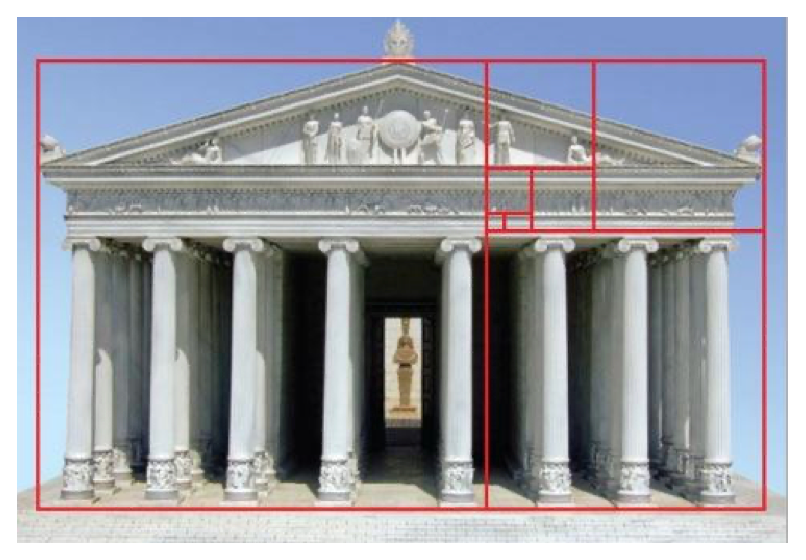
\includegraphics[width=4.5cm]{Parthenon}
\end{minipage}
\end{enigme}

\begin{corrige}
\begin{enumerate}
   \item Cette question est personnelle, cependant, {\blue le rectangle d} semble être le plus équilibré.
   \item Tableau complété : \\ \smallskip
   {\hautab{1.2}
      \small
      \begin{CLtableau}{\linewidth}{6}{c}
         \hline
         Rectangle & a & b & c & d & e \\
         \hline
         Length ($\ell$) in \ucm{} & 2 & 4 & 6 & 4 & 9 \\
         \hline
         Width ($w$) in \ucm{} & 2 & 2,5 & 2 & 2 & 1 \\
         \hline
         $\ell\div w$ & 1 & 1,6 & 3 & 2 & 9 \\
         \hline
      \end{CLtableau}}
   \item {\blue $10\div6,18 \approx 1,618$} et {\blue $6,18\div3,82 \approx 1,618$}.
   \item On trouve les dénominations suivantes : \\ 
      {\blue THE GOLDEN RATIO} ; \\
      {\blue THE GOLDEN PROPORTION} ; \\
      {\blue THE DIVINE PROPORTION} ; \\
      {\blue THE GOLDEN NUMBER}. \smallskip
   \item $\phi =\dfrac{1+\sqrt5}{2} \approx {\blue 1,618}$.
\end{enumerate}
\end{corrige}   

